\documentclass[10pt,openright,twoside,french]{book}

\input philippe2013
\input philippe2013_cours
\input philippe2013_sections
\input philippe2013_chapitre

\setcounter{chapter}{3}
\begin{document}

\renewcommand\PartProgramme{Géométrie}
\chapter[\'Equations de droites]{\'Equations de \\ droites}\label{ch_equations_droites}

On se place dans un repère orthonormé \OIJ.\par Une droite peut alors être parallèle à l'axe des ordonnées (cas n°1) ou bien sécante à l'axe des ordonnées (cas n°2).

\section{Caractérisation analytique d'une droite}\index{equation@équation!équation de droite}

\begin{minipage}{0.6\textwidth}
\textbf{Cas n°1 :} Une droite est parallèle à l'axe des ordonnées si et seulement si tous les points situés sur cette droite ont la même abscisse.

\begin{Prop}\index{equation@équation!équation réduite}
    Toute droite $(d)$ parallèle à l'axe des ordonnées a une équation \iptb{réduite} de la forme $x = k$ ($k \in \R$).
\end{Prop}
\end{minipage}%
\begin{minipage}{0.4\textwidth}
    \begin{center}
        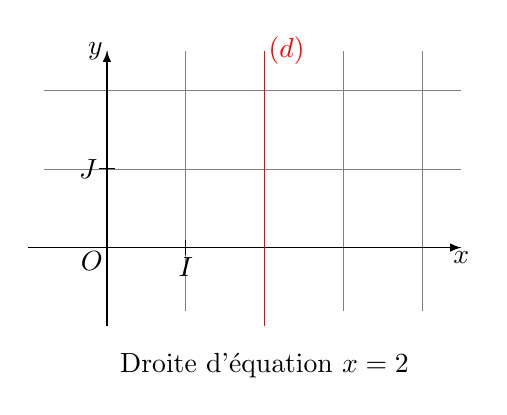
\begin{tikzpicture}[>=latex]
            \draw[help lines] (-0.8,-0.8) grid (4.5,2.5);
            \draw[->] (-1,0) -- (4.5,0) node[below=-2pt] {$x$};
            \draw[->] (0,-1) -- (0,2.5) node[left=-2pt] {$y$};
            \coordinate (O) at (0,0); \draw (O) node[below left = -2pt] {$O$};
            \coordinate (I) at (1,0); \draw (I) node[below] {$I$}; \draw (1,-0.1)--(1,0.1);
            \coordinate (J) at (0,1); \draw (J) node[left] {$J$}; \draw (-0.1,1)--(0.1,1);
            \draw[red] (2,-1) -- (2,2.5) node[right=-2pt] {$(d)$};
            \draw (2,-1.5) node {Droite d'équation $x = 2$};
        \end{tikzpicture}
    \end{center}
\end{minipage}

\begin{minipage}{0.6\textwidth}
\textbf{Cas n°2 :} Une droite qui coupe l'axe des ordonnées est la représentation d'une fonction affine. Réciproquement, une fonction affine a pour représentation graphique une droite sécante à l'axe des ordonnées.

\begin{Prop}\index{equation@équation!équation réduite}
    Toute droite $(d)$ sécante à l'axe des ordonnées a une équation \iptb{réduite} de la forme $y = mx + p$ ($m \in \R$ et $p \in \R$).
\end{Prop}
\end{minipage}%
\begin{minipage}{0.4\textwidth}
    \begin{center}
        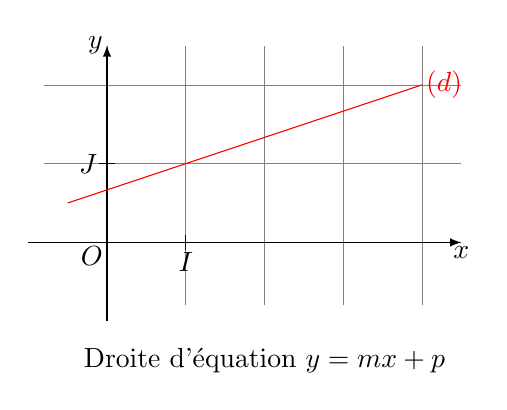
\begin{tikzpicture}[>=latex]
            \draw[help lines] (-0.8,-0.8) grid (4.5,2.5);
            \draw[->] (-1,0) -- (4.5,0) node[below=-2pt] {$x$};
            \draw[->] (0,-1) -- (0,2.5) node[left=-2pt] {$y$};
            \coordinate (O) at (0,0); \draw (O) node[below left = -2pt] {$O$};
            \coordinate (I) at (1,0); \draw (I) node[below] {$I$}; \draw (1,-0.1)--(1,0.1);
            \coordinate (J) at (0,1); \draw (J) node[left] {$J$}; \draw (-0.1,1)--(0.1,1);
            \draw[red] (-0.5,0.5) -- (4,2) node[right=-2pt] {$(d)$};
            \draw (2,-1.5) node {Droite d'équation $y = mx + p$};
        \end{tikzpicture}
    \end{center}
\end{minipage}

\begin{minipage}{0.6\textwidth}
\textbf{Cas particulier :} Lorsque $m = 0$, on trouve une équation de la forme $y = p$ ($p \in \R$). Dans ce cas, la droite $(d)$ est parallèle à l'axe des abscisses. Tous les points de cette droite ont la même ordonnée. Mais elle est toujours sécante à l'axe des ordonnées : c'est un cas particulier du cas n°2.
\end{minipage}%
\begin{minipage}{0.4\textwidth}
    \begin{center}
        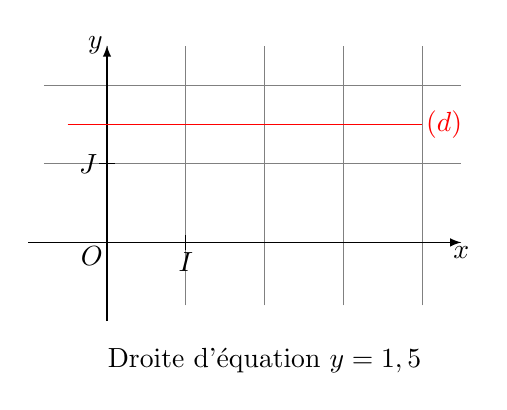
\begin{tikzpicture}[>=latex]
            \draw[help lines] (-0.8,-0.8) grid (4.5,2.5);
            \draw[->] (-1,0) -- (4.5,0) node[below=-2pt] {$x$};
            \draw[->] (0,-1) -- (0,2.5) node[left=-2pt] {$y$};
            \coordinate (O) at (0,0); \draw (O) node[below left = -2pt] {$O$};
            \coordinate (I) at (1,0); \draw (I) node[below] {$I$}; \draw (1,-0.1)--(1,0.1);
            \coordinate (J) at (0,1); \draw (J) node[left] {$J$}; \draw (-0.1,1)--(0.1,1);
            \draw[red] (-0.5,1.5) -- (4,1.5) node[right=-2pt] {$(d)$};
            \draw (2,-1.5) node {Droite d'équation $y = 1,5$};
        \end{tikzpicture}
    \end{center}
\end{minipage}

\begin{Defi}
    Considérons une droite $(d)$ dont l'équation réduite est de la forme : $y = mx + p$.\par
    Le nombre $m$ est appelé \ipt{c{\oe}fficient directeur} de la droite $(d)$. Ce \coef nous donne une indication sur l'inclinaison de la droite.\par
    Le nombre $p$ est appelé \ipt{ordonnée à l'origine}. En effet, lorsque $x = 0$ (origine de l'axe des abscisse), l'ordonnée $y$ est égale à $p$.
\end{Defi}

\section{Tracer une droite dans un repère}
Une droite d'équation $x = k$ passe par le point de coordonnées $(k \pv 0)$ et est parallèle à l'axe des ordonnées.\par
Une droite d'équation $y = p$ passe par le point de coordonnées $(0 \pv p)$ et est parallèle à l'axe des abscisses.\par
Pour représenter une droite d'équation $y = mx + p$, il faut et il suffit de connaître deux points appartenant à cette droite.

\begin{Exemple}[s]
    \begin{enumerate}
        \item Tracer la droite $(\Delta)$ d'équation $y = -2x + 3$.\par
        Puisqu'il faut deux points, choisissons arbitrairement deux valeurs de $x$ et calculons les valeurs de $y$ correspondantes.\par
        $x = 0$ : $y = -2 \times 0 + 3 = 3$ donc $A(0 \pv 3) \in (\Delta)$.\par
        $x = 1$ : $y = -2 \times 1 + 3 = 1$ donc $B(1 \pv 1) \in (\Delta)$.

        \item  Tracer la droite $(\Delta')$ d'équation $y = \frac 13 x - 1$.\par
        Puisqu'il faut deux points, choisissons arbitrairement deux valeurs de $x$ et calculons les valeurs de $y$ correspondantes.\par
        $x = 0$ : $y = \frac 13 \times 0 -1 = -1$ donc $C(0 \pv -1) \in (\Delta')$.\par
        $x = 3$ : $y = \frac13 \times 3 - 1 = 0$ donc $D(3 \pv 0) \in (\Delta)$.
    \end{enumerate}
        \begin{center}
            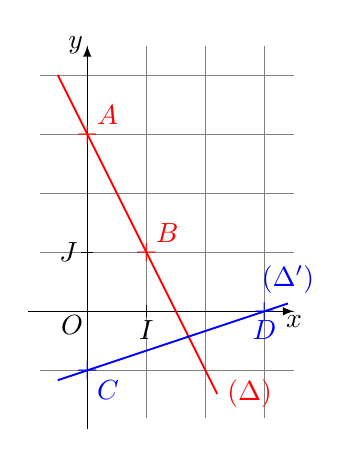
\begin{tikzpicture}[>=latex,scale=0.75]
                \draw[help lines] (-0.8,-1.8) grid (3.5,4.5);
                \draw[->] (-1,0) -- (3.5,0) node[below=-2pt] {$x$};
                \draw[->] (0,-2) -- (0,4.5) node[left=-2pt] {$y$};
                \coordinate (O) at (0,0); \draw (O) node[below left = -2pt] {$O$};
                \coordinate (I) at (1,0); \draw (I) node[below] {$I$}; \draw (1,-0.1)--(1,0.1);
                \coordinate (J) at (0,1); \draw (J) node[left] {$J$}; \draw (-0.1,1)--(0.1,1);
                \draw[color=red,line width=0.7pt] plot[domain=-0.5:2.2,samples=200] (\x,{-2*\x+3}) node[right] {$(\Delta)$};
                \draw[red] (0,3) node {$+$} node[above right] {$A$};
                \draw[red] (1,1) node {$+$} node[above right] {$B$};
                \draw[color=blue,line width=0.7pt] plot[domain=-0.5:3.4,samples=200] (\x,{\x/3-1}) node[above] {$(\Delta')$};
                \draw[blue] (0,-1) node {$+$} node[below right] {$C$};
                \draw[blue] (3,0) node {$+$} node[below] {$D$};
            \end{tikzpicture}
        \end{center}
\end{Exemple}

\section{Déterminer l'équation d'une droite}
\subsection{Cas n°1}
Une droite parallèle à l'axe des ordonnées a pour équation $x = k$.\par
Si on connaît la représentation graphique de la droite, il suffit ensuite de lire graphiquement la valeur de $k$. Sinon, en connaissant deux points, il suffit de lire leur abscisse commune.\medskip

\begin{Exemple}
    Déterminer l'équation de la droite passant par les points $K(-2 \pv 3)$ et $L(-2 \pv 6)$.\par
    Ces deux points ont la même abscisse donc la droite $(KL)$ est parallèle à l'axe des ordonnées et a pour équation $x = -2$.
\end{Exemple}

\subsection{Cas n°2}
Une droite sécante à l'axe des ordonnées à une équation de la forme $y = mx + p$. Deux points situés sur cette droite n'ont pas la même abscisse.\par

Lorsque l'on connaît les coordonnées de deux points de la droite, on détermine d'abord le \coef directeur puis on résoud une équation pour déterminer l'ordonnée à l'origine.

\begin{Prop}
    Soient $K(x_K \pv y_K)$ et $L(x_L \pv y_L)$ deux points dans un repère tel que $x_K \neq x_L$.\par
    Le \coef directeur de la droite $(KL)$ est : \[m = \frac{y_K - y_L}{x_K - x_L}.\]
\end{Prop}\clearpage

\begin{Demo}
    $K \in (KL)$ donc $y_K = mx_K + p$. De même, puisque $L \in (KL)$ alors $y_L = mx_L + p$.\par
    Ainsi,
    $\begin{array}[t]{rcl}
        y_K - y_L & = & mx_K + p - (mx_L + p)\\ &=& mx_K + p - mx_L - p\\ &=& mx_K - mx_L\\ &=& m(x_K - x_L)\end{array}$\medskip

        Puisque $x_K \neq x_L$, alors $x_K - x_L \neq 0$ et en divisant par $x_K - x_L$, on obtient :
        \[m = \frac{y_K - y_L}{x_K - x_L}.\]
\end{Demo}

\begin{Rmq}
    Lorsque l'on passe d'un point d'une droite à une autre en augmentant l'abscisse de $1$, alors la variation des ordonnées est donnée par $m$.
\end{Rmq}

\begin{Exemple}
    Déterminer l'équation de la droite $(d)$ passant par les points $A(3 \pv 4)$ et $(5 \pv -2)$.\par\medskip
    Les deux points n'ont pas la même abscisse donc l'équation réduite de la droite $(d)$ est de la forme $y = mx + p$.\par
    \begin{multicols}{2}
    \begin{description}
        \item[Calcul de $m$ :] $\begin{array}[t]{rcl}
                                                    m & = & \frac{y_A - y_B}{x_A - x_B}\\[10pt]
                                                        & = & \frac{4 - (-2)}{3 - 5}\\[10pt]
                                                        & = & \frac{6}{-2}\\[10pt]
                                                    m &= & -3
                                                \end{array}$
        \item[Calcul de $p$ :] Puisque $A \in (d)$ alors les coordonnées de $A$ vérifient l'équation de $(d)$ :
        \[\begin{array}{ll}
            & y_A = mx_A + p \\
            \Leftrightarrow & 4 = -3 \times 3 + p \\
            \Leftrightarrow & 4 = -9 + p \\
            \Leftrightarrow & p = 4 + 9 \\
            \Leftrightarrow & p = 13
        \end{array}\]
    \end{description}
        \end{multicols}
        La droite $(d)$ a donc pour équation : $y = -3x + 13$.
\end{Exemple}

\begin{Exemple}
    Déterminer l'équation de la droite $(d')$ dont voici la représentation graphique.

        \begin{center}
            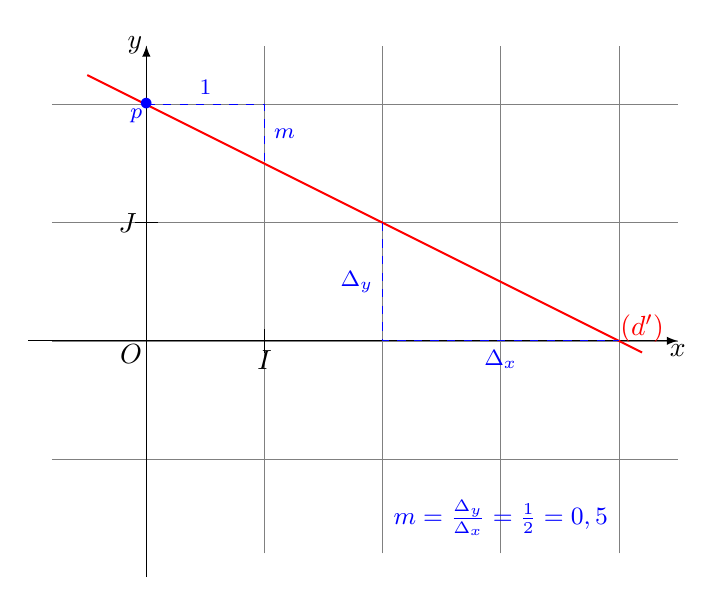
\begin{tikzpicture}[>=latex,scale=1.5]
                \draw[help lines] (-0.8,-1.8) grid (4.5,2.5);
                \draw[->] (-1,0) -- (4.5,0) node[below=-2pt] {$x$};
                \draw[->] (0,-2) -- (0,2.5) node[left=-2pt] {$y$};
                \coordinate (O) at (0,0); \draw (O) node[below left = -2pt] {$O$};
                \coordinate (I) at (1,0); \draw (I) node[below] {$I$}; \draw (1,-0.1)--(1,0.1);
                \coordinate (J) at (0,1); \draw (J) node[left] {$J$}; \draw (-0.1,1)--(0.1,1);
                \draw[color=red,line width=0.7pt] plot[domain=-0.5:4.2,samples=200] (\x,{-0.5*\x+2}) node[above] {$(d')$};
                \draw[blue, dashed] (0,2) -- (1,2) node[above,midway] {\footnotesize $1$} -- (1,1.5) node[right,midway] {\footnotesize $m$};
                \draw[blue, dashed] (2,1) -- (2,0) node[left,midway] {\footnotesize $\Delta_y$} -- (4,0) node[below,midway] {\footnotesize $\Delta_x$};
                \draw[blue] (0,2) node{$\bullet$} node[below left = -2pt] {\footnotesize $p$};
                \draw[blue] (3,-1.5) node {\small $m = \frac{\Delta_y}{\Delta_x} = \frac 12 = 0,5$};
            \end{tikzpicture}
        \end{center}
        La droite $(d')$ a pour équation : $y = \frac 1 2 x + 2$.
\end{Exemple}\clearpage

\section{Applications}
\subsection{Droites parallèles}
\begin{Rmq}[s]
    \begin{enumerate}
        \item Les droites qui ont une équation de la forme $x = k$ sont toutes parallèles à l'axe des ordonnées et elles sont donc parallèles entre elle.
        \item Une droite d'équation $x = k$ et une droite d'équation $y = mx + p$ sont sécantes car la première est parallèle à l'axe des ordonnées et pas la suivante.
    \end{enumerate}
\end{Rmq}

\begin{Prop}
    Une droite $(d)$ d'équation $y = mx + p$ et une droite $(d')$ d'équation $y = m'x + p'$ sont parallèles si, et seulement si, elles ont le même \coef directeur :
    \[(d) /\!/ (d') \quad \Leftrightarrow \quad m = m'\]
\end{Prop}

\begin{Demo}
On se place dans la situation suivante : les points $A$ et $B$ appartient à la droite $(d)$ et les points $A'$ et $B'$ appartiennent à la droite $(d')$ tels que $(AA') /\!/ (BB')$.
\begin{center}
    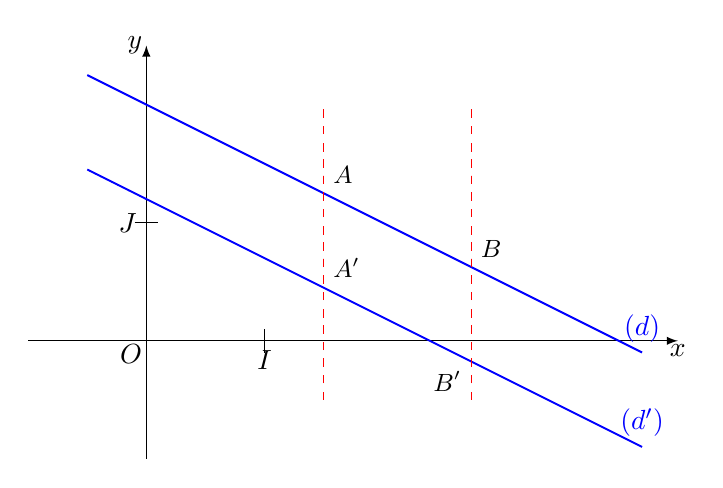
\begin{tikzpicture}[>=latex,scale=1.5]
        \draw[->] (-1,0) -- (4.5,0) node[below=-2pt] {$x$};
        \draw[->] (0,-1) -- (0,2.5) node[left=-2pt] {$y$};
        \coordinate (O) at (0,0); \draw (O) node[below left = -2pt] {$O$};
        \coordinate (I) at (1,0); \draw (I) node[below] {$I$}; \draw (1,-0.1)--(1,0.1);
        \coordinate (J) at (0,1); \draw (J) node[left] {$J$}; \draw (-0.1,1)--(0.1,1);
        \draw[color=blue,line width=0.7pt] plot[domain=-0.5:4.2,samples=200] (\x,{-0.5*\x+2}) node[above] {$(d)$};
        \draw[color=blue,line width=0.7pt] plot[domain=-0.5:4.2,samples=200] (\x,{-0.5*\x+1.2}) node[above] {$(d')$};
        \draw[color=red,dashed] plot[domain=-0.5:2,samples=200] (1.5,\x);
        \draw[color=red,dashed] plot[domain=-0.5:2,samples=200] (2.75,\x);
        \draw (1.5,1.25) node[above right] {\small$A$}; \draw (2.75,0.625) node[above right] {\small$B$};
        \draw (1.5,0.45) node[above right] {\small$A'$}; \draw (2.75,-0.175) node[below left] {\small$B'$};
    \end{tikzpicture}
\end{center}

\renewcommand\arraystretch{1.75}
\begin{tabular}{ll}
    & $(d)$ et $(d')$ sont parallèles \\
    $\Leftrightarrow$ & $ABB'A'$ est un parallélogramme \\
    $\Leftrightarrow$ & $[AB']$ et $[A'B]$ ont le même milieu \\
    $\Leftrightarrow$ & $\left\{\begin{array}{rcl} \frac{x_A + x_{B'}}{2} = \frac{x_{A'} + x_{B}}{2} \\[7pt] \frac{y_A + y_{B'}}{2} = \frac{y_{A'} + y_{B}}{2} \end{array}\right.$ \\
    $\Leftrightarrow$ & $\left\{\begin{array}{rcl} x_A + x_{B'} = x_{A'} + x_{B} \\ y_A + y_{B'} = y_{A'} + y_{B} \end{array}\right.$ \\
    $\Leftrightarrow$ & $\left\{\begin{array}{rcl} x_A - x_{B} = x_{A'} - x_{B'} \\ y_A - y_{B} = y_{A'} - y_{B'} \end{array}\right.$ \\
    $\Leftrightarrow$ & $\frac{y_B - y_A}{x_B - x_A} = \frac{y_{B'} - y_{A'}}{x_{B' }- x_{A'}}$\qquad (équivalence car $x_A = x_{A'}$ et $x_B = x_B'$)\\
    $\Leftrightarrow$ & $m = m'$
\end{tabular}
\renewcommand\arraystretch{1}

On a bien démontré que $(d) /\!/ (d') \quad \Leftrightarrow \quad m = m'$.
\end{Demo}

\begin{Exemple}
    Donner les équations réduites des droites suivantes et déterminer celles qui sont parallèles :
    \[(d_1) : y - 2x + 1 = 0 \qq (d_2) : y + 3x - 2 = 0 \qq (d_3) : 4y + 12x - 20 = 0 \qq (d_4) : y + 1 = 2x.\]
\end{Exemple}

\subsection{Droites sécantes}
Soient $(d)$ d'équation $y = mx + p$ et $(d')$ d'équation $y = m'x + p'$. D'après la propriété précédente, deux droites sont sécantes lorsque $m \neq m'$.
Dans ce cas, il existe un point d'intersection $A$ et les coordonnées de $A$ vérifient les équations des deux droites en même temps. On a donc le système suivant dont le couple $(x \pv y)$ est l'inconnue qui correspond aux coordonnées du point $A$ :
\[\left\{\begin{array}{l} y = mx + p \\y = m'x + p' \end{array}\right.\]

\begin{Exemple}
Déterminer les coordonnées du point d'intersection des droites suivantes :
\[(\Delta_1) : y = -2x + 3 \qq (\Delta_2) : y = \frac 13 x - 1\]
\end{Exemple}

\subsection{Alignement de points}

\begin{Prop}
    On considère trois points $A$, $B$ et $C$.
    \begin{enumerate}
        \item Si les trois points ont la même abscisse $k$, alors ils sont alignés.
        \item Sinon, les points sont alignés si et seulement si $(AB)$ et $(AC)$ ont le même \coef directeur.
    \end{enumerate}
\end{Prop}

\begin{Demo}
    Dans le premier cas, les points appartiennent à la même droite d'équation $x = k$ donc ils sont alignés.\par
    Dans le second cas, dire que $(AB)$ et $(AC)$ ont le même \coef directeur est équivalent à dire que ces droites sont parallèles ce qui est équivalent à dire qu'elles sont confondues (puisqu'elles ont un point commun) ce qui équivaut à dire qu'il s'agit de la même droite et donc $A$, $B$ et $C$ sont alignés.
\end{Demo}

\begin{Exemple}
    Dans chacun des cas, les points $A$, $B$ et $C$ sont-ils alignés ?
    \[A(6 \pv 0) \qq B(0 \pv 4) \qq C(3 \pv 2)\]\[A(1 \pv 3) \qq B(2 \pv 9) \qq C(4 \pv 10)\]
\end{Exemple}
\end{document}
